\documentclass[aspectratio=169]{beamer}
\usepackage[T1]{fontenc}
\usepackage[utf8]{inputenc}
\usepackage{tikz}
\usepackage{tabularx}
\usepackage[font=scriptsize]{caption}
\captionsetup[figure]{labelformat=empty}

\usetikzlibrary{tikzmark,shapes,arrows,backgrounds,fit,positioning}
\newcolumntype{C}{>{\centering\arraybackslash}X}

\addtobeamertemplate{navigation symbols}{}{
	\insertframenumber{}
	}

\title{SDEU Baseline}
\author{
  Mauricio Su\'arez Dur\'an and Ioana~C.~Mari\c{s}
}
\institute{IIHE-ULB}

\titlegraphic{
  \begin{figure}[h]
    \centering
   
\includegraphics[width=5cm]{ulbLogo2.png}
    \hspace*{2.cm}
    
\includegraphics[width=5.5cm]{iihe.jpeg}
  \end{figure}
}

\begin{document}
\begin{frame}
  \titlepage
\end{frame}

\begin{frame}
  \begin{itemize}
    \item Baseline stability for pre-production batch of UUBs together with SPMT and SSD in the field.
    \item Data from CDAS: from 01/12/2020 to 28/02/2021
  \end{itemize}
  \begin{figure}
    \centering
    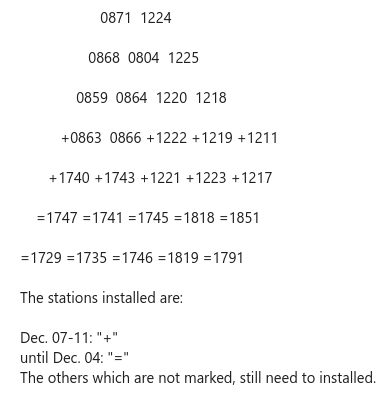
\includegraphics[width=.35\textwidth]{listStations.png}
  \end{figure}
\end{frame}


\begin{frame}
	Trace selection method
  \begin{figure}[h]
    \centering
    \includegraphics[width=0.85\textwidth]{../plots/sglEvt.pdf}
	\end{figure}

	\begin{tikzpicture}[overlay,remember picture]
		\path (current page.south west) +(0.1*pi,pi) 
		node[text width=13cm,anchor=south west]{\begin{alignat}{2}
			\mathrm{First\, 100\, bins} \quad \quad \quad \quad \quad
			\qquad \qquad \qquad
			\mathrm{Last\, 100\, bins} \nonumber
		\end{alignat}};
	\end{tikzpicture}

\end{frame}


\begin{frame}
	RMS difference for traces that agree with: $\mid \mathrm{Mean}_f - \mathrm{Mean}_l \mid < 2\left( \mathrm{RMS_f} \right) $

  \centering
	\includegraphics[width=.49\textwidth]{../plots/trOkPMT1Hg.pdf}\quad%
	\begin{minipage}[b][0.4\textheight][c]
		{.45\linewidth}
	\end{minipage}\\[1em]
	\includegraphics[width=.48\textwidth]{../plots/trOkPMT2Hg.pdf}\quad%
	\includegraphics[width=.48\textwidth]{../plots/trOkPMT3Hg.pdf}
\end{frame}


\begin{frame}
	1851 station's PMT3 HG

  \centering
	\includegraphics[width=.48\textwidth]{../plots/traces1851Pmt3.png}
	\includegraphics[width=.48\textwidth]{../plots/traces1851FLPmt3.pdf}
\end{frame}


\begin{frame}
	Distrubition of RMS for the last 100 bins of station 1851
	\centering
	\includegraphics[width=1.\textwidth]{../plots/rmsDistriPmt1851.pdf}
\end{frame}


\begin{frame}
	\frametitle{Charge Histograms, Station 863}	
	\begin{figure}
		\begin{tabularx}{\textwidth}{CCC}
			\multicolumn{3}{l}{From IoSdHisto method}	
			\\
			\includegraphics[width=.3\textwidth]{../plots/chargeHChargePMT1.pdf}
			&
			\includegraphics[width=.3\textwidth]{../plots/chargeHChargePMT2.pdf}
			&
			\includegraphics[width=.3\textwidth]{../plots/chargeHChargePMT3.pdf}
			\\ 
			\multicolumn{3}{l}{From IoSdStation::HCharge method: }
			\\
			\multicolumn{3}{l}{xc[j] = mult*j + offset; xc[400+j] = 400*mult + bigbins*mult*j + offset} 
			\\ [2ex]
			\includegraphics[width=.3\textwidth]{../plots/chargeHistoPMT1.pdf}
			&
			\includegraphics[width=.3\textwidth]{../plots/chargeHistoPMT2.pdf}
			&
			\includegraphics[width=.3\textwidth]{../plots/chargeHistoPMT3.pdf}
		\end{tabularx}
	\end{figure}
\end{frame}


\begin{frame}
	\frametitle{Peak Histograms, Station 863}	
	\begin{figure}
		\begin{tabularx}{\textwidth}{CCC}
			\multicolumn{3}{l}{From IoSdHisto method}	
			\\
			\includegraphics[width=.3\textwidth]{../plots/peakHPeakPMT1.pdf}
			&
			\includegraphics[width=.3\textwidth]{../plots/peakHPeakPMT2.pdf}
			&
			\includegraphics[width=.3\textwidth]{../plots/peakHPeakPMT3.pdf}
			\\ 
			\multicolumn{3}{l}{From IoSdStation::HPeak method: }
			\\
			\multicolumn{3}{l}{xc[j] = mult*j + offset; xc[400+j] = 400*mult + bigbins*mult*j + offset} 
			\\ [2ex]
			\includegraphics[width=.3\textwidth]{../plots/peakHistoPMT1.pdf}
			&
			\includegraphics[width=.3\textwidth]{../plots/peakHistoPMT2.pdf}
			&
			\includegraphics[width=.3\textwidth]{../plots/peakHistoPMT3.pdf}
		\end{tabularx}
	\end{figure}
\end{frame}


\begin{frame}
	Averages histograms for Station 863:
	\begin{figure}
		\begin{tabularx}{\textwidth}{CCC}
			\includegraphics[width=4.15cm]{../plots/uubAveChHistoPMT1St863.pdf}
			\caption{Charge UUB-LPMT1}
			&
			\includegraphics[width=4.15cm]{../plots/uubAveChHistoPMT2St863.pdf}
			\caption{Charge UUB-LPMT2}
			&
			\includegraphics[width=4.15cm]{../plots/uubAveChHistoPMT3St863.pdf}
			\caption{Charge UUB-LPMT3}
			\\ [2ex]
			\includegraphics[width=4.15cm]{../plots/uubAvePkHistoPMT1St863.pdf}
			\caption{Peak UUB-LPMT1}
			&
			\includegraphics[width=4.15cm]{../plots/uubAvePkHistoPMT2St863.pdf}
			\caption{Peak UUB-LPMT2}
			&
			\includegraphics[width=4.15cm]{../plots/uubAvePkHistoPMT3St863.pdf}
			\caption{Peak UUB-LPMT3}
			\end{tabularx}
	\end{figure}
\end{frame}


























\begin{frame}
	\frametitle{Area/Peak inspection}
	Fitting Histograms using:
	\begin{displaymath}
		e^{\left( a_0-\frac{1}{x\tau}\right) } + x^{-1}e^{ -\left(\frac{(\ln x - \ln\mu)^2}{2\sigma^2}\right) }
	\end{displaymath}
	Charge histogram for Station 1223
	\vspace{0.5cm}
	
	\begin{figure}
		\begin{tabularx}{\textwidth}{CCC}
			\includegraphics[width=.35\textwidth]{../plots/ubChHistFitSt1223.pdf}
			\caption{Charge: UB-PMT1}
			&
			\includegraphics[width=.35\textwidth]{../plots/uubChHistFitSt1223.pdf}
			\caption{Charge: UUB-PMT1}
			&
			\includegraphics[width=.35\textwidth]{../plots/ubPkHistFitSt1222.pdf}
			\caption{Peak: UUB-PMT1}
		\end{tabularx}
	\end{figure}
\end{frame}


\begin{frame}
	Position of VEM-Charge, average per day, traces agree with: $\mid \mathrm{M}_f - \mathrm{M}_l \mid < 2\left( \mathrm{RMS_f} \right) $

  \centering
	\includegraphics[width=.49\textwidth]{../plots/uuBchargePMT1Hg.pdf}\quad%
	\begin{minipage}[b][0.4\textheight][c]
		{.45\linewidth}
	\end{minipage}\\[1em]
	\includegraphics[width=.48\textwidth]{../plots/uuBchargePMT2Hg.pdf}\quad%
	\includegraphics[width=.48\textwidth]{../plots/uuBchargePMT3Hg.pdf}
\end{frame}


\begin{frame}
	Position of VEM-Peak, average per day, traces agree with: $\mid \mathrm{M}_f - \mathrm{M}_l \mid < \left( 2*\mathrm{RMS_f} \right) $

  \centering
	\includegraphics[width=.49\textwidth]{../plots/uuBpeakPMT1Hg.pdf}\quad%
	\begin{minipage}[b][0.4\textheight][c]
		{.45\linewidth}
	\end{minipage}\\[1em]
	\includegraphics[width=.48\textwidth]{../plots/uuBpeakPMT2Hg.pdf}\quad%
	\includegraphics[width=.48\textwidth]{../plots/uuBpeakPMT3Hg.pdf}
\end{frame}


\begin{frame}
	A/P average per day, traces that agree with: $\mid \mathrm{Mean}_f - \mathrm{Mean}_l \mid < 2\left( \mathrm{RMS_f} \right) $

  \centering
	\includegraphics[width=.49\textwidth]{../plots/uuBapPMT1Hg.pdf}%\quad%
	\begin{minipage}[b][0.2\textheight][c]
		{.15\linewidth}
	\end{minipage}\\[1em]
	\includegraphics[width=.48\textwidth]{../plots/uuBapPMT2Hg.pdf}\quad%
	\includegraphics[width=.48\textwidth]{../plots/uuBapPMT3Hg.pdf}
\end{frame}


\begin{frame}
	\frametitle{A/P along UB and UUB}
	
	\begin{figure}
		\begin{tabularx}{\textwidth}{CCC}
			\includegraphics[width=.37\textwidth]{../plots/areaPeakTimePMT1St863.pdf}
			&
			\includegraphics[width=.37\textwidth]{../plots/areaPeakTimePMT1St1741.pdf}
			&
			\includegraphics[width=.37\textwidth]{../plots/areaPeakTimePMT1St1819.pdf}
			\\ [2ex]
			\includegraphics[width=.37\textwidth]{../plots/areaPeakTimePMT2St1219.pdf}
			&
			\includegraphics[width=.37\textwidth]{../plots/areaPeakTimePMT3St1222.pdf}
			&
			\includegraphics[width=.37\textwidth]{../plots/areaPeakTimePMT3St1851.pdf}
		\end{tabularx}
	\end{figure}
\end{frame}


\begin{frame}
  \centering
	{\Huge\bf\it Thanks}
\end{frame}

% ========================================================
% ****************** BACKUP SLIDES ***********************
% ========================================================

\begin{frame}
  \centering
	{\Huge\bf\it Backup}
\end{frame}


\begin{frame}
	Averages histograms for Station 1223 (since december):
	\begin{figure}
		\begin{tabularx}{\textwidth}{CCC}
			\includegraphics[width=4.15cm]{../plots/ubAveChHistoPmt1St1223.pdf}
			\caption{UB-LPMT1}
			&
			\includegraphics[width=4.15cm]{../plots/ubAveChHistoPmt2St1223.pdf}
			\caption{UB-LPMT2}
			&
			\includegraphics[width=4.15cm]{../plots/ubAveChHistoPmt3St1223.pdf}
			\caption{UB-LPMT3}
			\\ [-2ex]
			\includegraphics[width=4.15cm]{../plots/uubAveChHistoPMT1St1223.pdf}
			\caption{UUB-LPMT1}
			&
			\includegraphics[width=4.15cm]{../plots/uubAveChHistoPMT2St1223.pdf}
			\caption{UUB-LPMT2}
			&
			\includegraphics[width=4.15cm]{../plots/uubAveChHistoPMT3St1223.pdf}
			\caption{UUB-LPMT3}
			\end{tabularx}
	\end{figure}
\end{frame}


\begin{frame}
	Averages histograms for Station 1851:
	\begin{figure}
		\begin{tabularx}{\textwidth}{CCC}
			\includegraphics[width=4.15cm]{../plots/ubAveChHistoPmt1St1851.pdf}
			\caption{UB-LPMT1}
			&
			\includegraphics[width=4.15cm]{../plots/ubAveChHistoPmt2St1851.pdf}
			\caption{UB-LPMT2}
			&
			\includegraphics[width=4.15cm]{../plots/ubAveChHistoPmt3St1851.pdf}
			\caption{UB-LPMT3}
			\\ [-2ex]
			\includegraphics[width=4.15cm]{../plots/uubAveChHistoPmt1St1851.pdf}
			\caption{UUB-LPMT1}
			&
			\includegraphics[width=4.15cm]{../plots/uubAveChHistoPmt2St1851.pdf}
			\caption{UUB-LPMT2}
			&
			\includegraphics[width=4.15cm]{../plots/uubAveChHistoPmt3St1851.pdf}
			\caption{UUB-LPMT3}
			\end{tabularx}
	\end{figure}
\end{frame}


\begin{frame}
	{\bf UB:} A/P average per day, traces that agree with: $\mid \mathrm{Mean}_f - \mathrm{Mean}_l \mid < \left( 2*\mathrm{RMS_f} \right) $

  \centering
	\includegraphics[width=.45\textwidth]{../plots/uBapPMT1Hg.pdf}%\quad%
	\begin{minipage}[b][0.2\textheight][c]
		{.15\linewidth}
	\end{minipage}\\[1em]
	\includegraphics[width=.45\textwidth]{../plots/uBapPMT2Hg.pdf}\quad%
	\includegraphics[width=.45\textwidth]{../plots/uBapPMT3Hg.pdf}
\end{frame}


\end{document}
